\documentclass[12pt]{article}

\usepackage[margin=1in]{geometry}
\usepackage{amsmath}
\usepackage{amssymb}
\usepackage{physics}
\usepackage{array}
\usepackage{graphicx}

\title{Voltage and EMF Calculations}
\author{Saraansh Wadkar}
\date{}

\begin{document}

\maketitle

\section{Applied motor equation}

\[
V_{\text{applied}} = I_{\text{motor}} \cdot R + k_e \cdot \omega
\]

\par $I_{\text{motor}} \cdot R$ is the voltage that's needed to target a current through resistance. When we targetting a current in current control $I_{\text{motor}}$ is what we're targetting.
\par $k_e \cdot \omega$ is the back-emf that results from the motor spinning. For the motor to not act like a generator, we need to counteract the back-emf hence it being part of our applied equation. Note that $k_e \cdot \omega$ has its angular velocity units cancel out here and so this ends up contributing $V$ to the applied voltage equation.

\subsection{When $\omega = 0$}
When we stall, our motor doesn't move at all. This means that our applied voltage can be represented by:
$$
\begin{aligned}
V_{\text{applied}} \mid_{\omega=0} &= I_{\text{motor}} \cdot R + k_e \cdot \omega \mid_{\omega=0}\\  &= I_{\text{motor}} \cdot R
\end{aligned}
$$
This means that when we are stalling ($\omega = 0$) then we apply no voltage to counteract the back-emf. So our voltage applied strictly becomes a function of the current we choose to target.

\par Also recall that torque is proportional to current because:
$$
\tau = k_t \cdot I \rightarrow I = \frac{\tau}{k_t}
$$

So since current is proportional to torque, in the case where we are stalling, we can achieve a relatively high torque to applied voltage ratio as:
$$
V_{\text{applied}} \mid_{\omega = 0} = I_{\text{motor}} \cdot R = \frac{\tau}{k_t} \cdot R
$$

Where the internal resistance of a motor is fairly low. TLDR: High torque, low voltage when stalling, which is good for situations in which we're stuck because we're not consuming a lot of power here ($P = V \cdot I$) and eating up our battery.

\subsection{When $\omega \neq 0$}
When $\omega \neq 0$ now the back-emf actually does matter to us, and at higher speeds, most of our voltage is going to go towards counteracting our back-emf. Let's say at some point we hit such a high free speed such that:
$$
k_e \cdot \omega = 12V
$$

Recall our voltage applied equation:
$$
V_{\text{applied}} = I_{\text{motor}} \cdot R + k_e \cdot \omega
$$

Substituting our high free speed motor that needs 12V to counteract back-emf:
$$
V_{\text{applied}} = I_{\text{motor}} \cdot R + 12V
$$

Since we can only physically apply as much voltage as we are supplied (in FRC it's from our 12V battery), we cannnot request any current here. So since $I = 0 \rightarrow \tau = 0$ which means we have no torque.

\subsection{Why applying constant current solves our issues}
The core issue with voltage control is that we are not directly controlling torque. Motor torque is proportional to motor current:
\[
\tau = k_t \cdot I
\]
so when current changes, torque changes with it.

\par That is a problem for an intake because the operating condition changes a lot. When the intake is moving, some of the applied voltage must go toward canceling back-emf:
\[
V_{\text{applied}} = I_{\text{motor}} \cdot R + k_e \cdot \omega
\]
But when the intake stalls, $\omega \to 0$, so the back-emf term disappears:
\[
V_{\text{applied}} \mid_{\omega = 0} = I_{\text{motor}} \cdot R
\]
Under voltage control, this means the same commanded voltage can produce very different current depending on speed. At stall, the current can spike and produce too much torque. While moving, back-emf consumes more of the available voltage, so current falls and we may get too little torque.

\par Constant current control fixes this because it regulates the quantity that directly sets torque. If we choose a target current $I_{\text{target}}$, then our torque is approximately:
\[
\tau \approx k_t \cdot I_{\text{target}}
\]
At stall, where there is no back-emf, the controller only applies enough voltage to hold that chosen current:
\[
V_{\text{applied}} \mid_{\omega = 0} = I_{\text{target}} \cdot R
\]
So instead of surging to a large stall current, the motor is held to a safe current and therefore a safe torque.

\par When the intake is moving, the controller automatically raises the applied voltage to overcome back-emf while still maintaining the same current target:
\[
V_{\text{applied}} = I_{\text{target}} \cdot R + k_e \cdot \omega
\]
This gives us a more consistent torque across changing operating conditions. TLDR here is that:
\par When we stall, current control prevents an unsafe current spike and limits torque to a safe value
\par When we are moving, current control compensates for back-emf so torque does not fall off as much

\par This is why constant current is effectively constant torque control for the intake: it makes the mechanism behave more predictably both when it is freely moving and when it gets stuck.

\subsubsection{A perfectly tuned voltage controller could do the same thing in theory}
In theory, a voltage controller could produce the exact same torque output as a current controller if it had an accurate model of the motor and continuously updated its voltage command from that model.

\par Start with the motor equation:
\[
I = \frac{V_{\text{applied}} - k_e \cdot \omega}{R}
\]
and recall that motor torque is proportional to current:
\[
\tau = k_t \cdot I
\]
Substituting the current equation into the torque equation gives:
\[
\tau = k_t \cdot \frac{V_{\text{applied}} - k_e \cdot \omega}{R}
\]

\par If we instead start from a desired torque $\tau_{\text{target}}$, then the equivalent desired current is:
\[
I_{\text{target}} = \frac{\tau_{\text{target}}}{k_t}
\]
and solving the motor equation for the required applied voltage gives:
\[
V_{\text{applied}} = I_{\text{target}} \cdot R + k_e \cdot \omega
\]
So yes: in principle, if we constantly measured motor speed $\omega$ and continually updated $V_{\text{applied}}$ using this equation, then a voltage controller could command the same torque that a current controller would command.

\par The reason current control is simpler is that it removes most of this inversion work from the high-level controller. Torque is directly proportional to current, so if we want a certain torque, we can command the corresponding current and let the current loop handle whatever applied voltage is necessary to achieve it. The current controller automatically increases voltage when back-emf is high and reduces voltage when back-emf is low.

\par So the distinction is:
\par Voltage control for constant torque: estimate $\omega$, compute the needed voltage, and keep updating that voltage as conditions change
\par Current control for constant torque: command the desired current directly, since current is already proportional to torque

\par This is why current control is usually the cleaner abstraction. It gives us a control input that maps much more directly to the physical quantity we care about.

% \begin{figure}[h]
% \centering
% 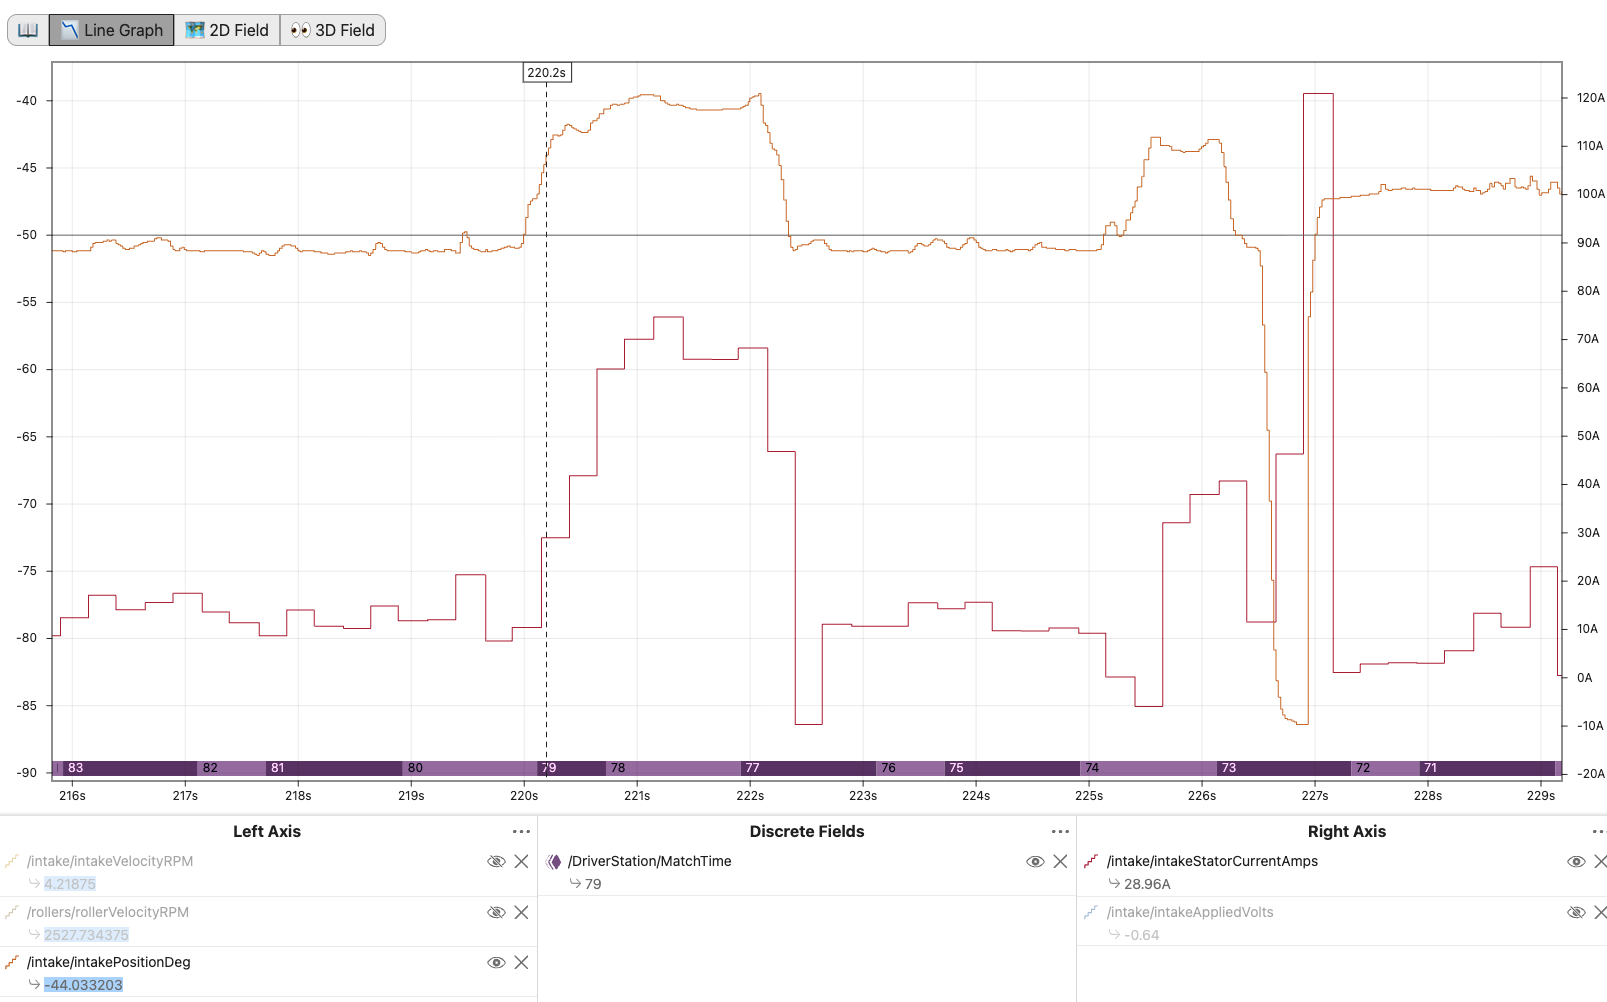
\includegraphics[width=\textwidth]{assets/degvsstator.png}
% \caption{Intake position versus stator current. The current changes noticeably through the event, which means the produced torque changes noticeably as well.}
% \end{figure}

\begin{figure}[h]
\centering
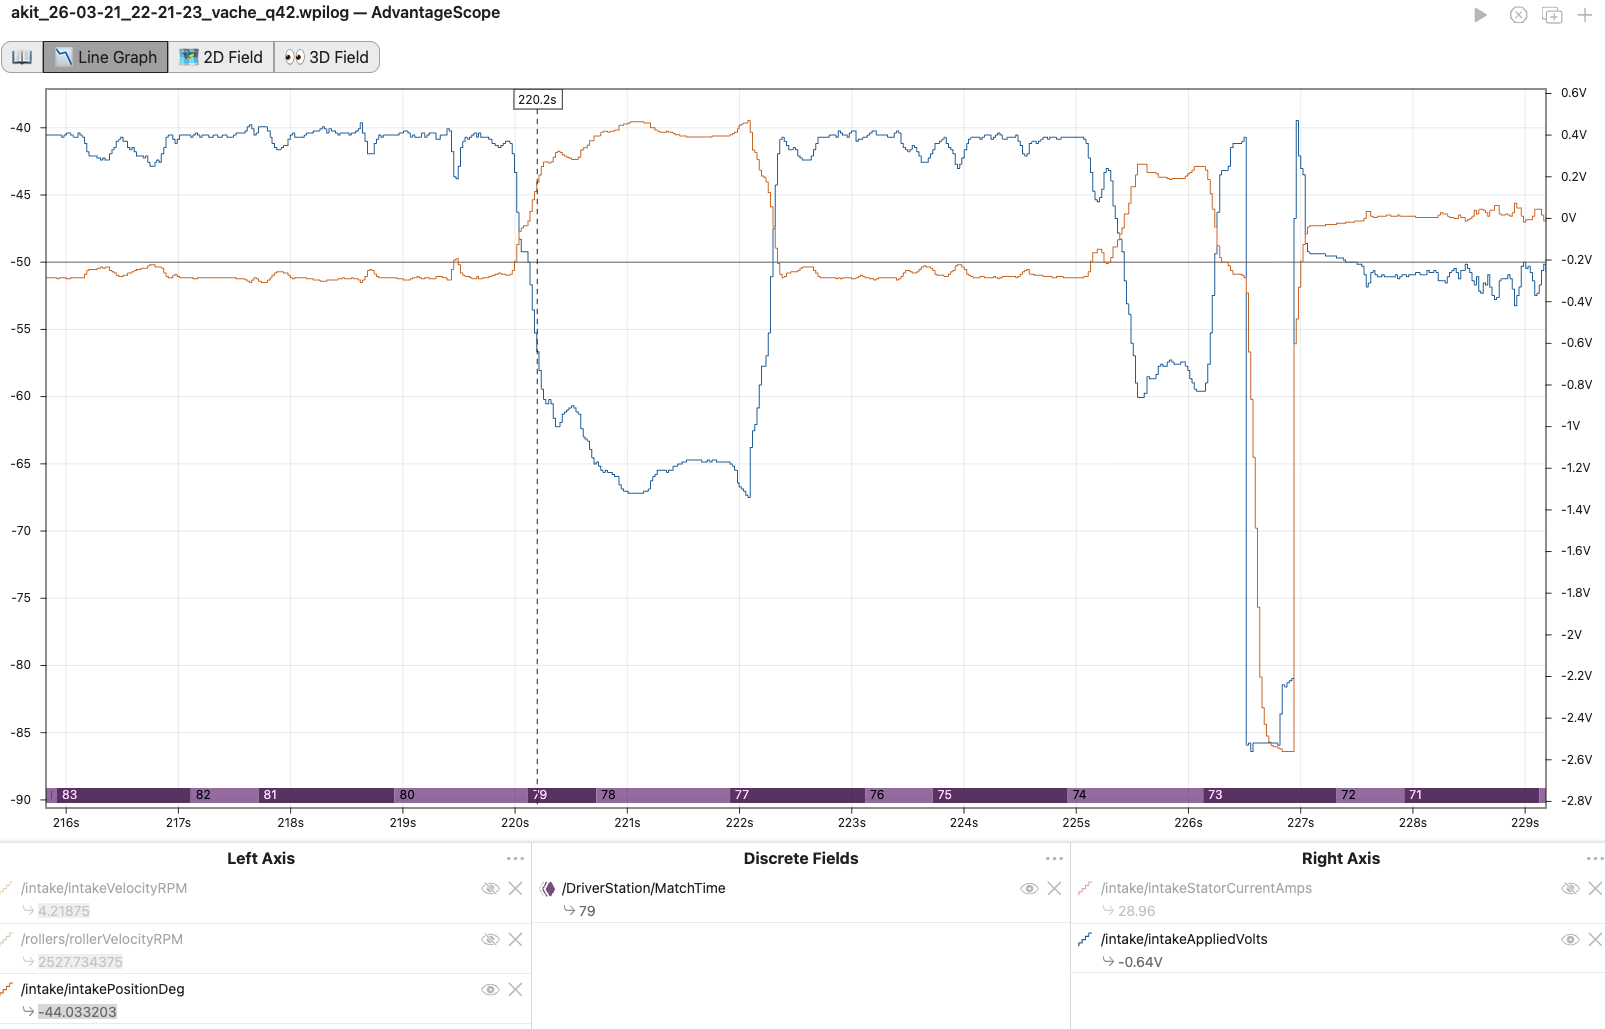
\includegraphics[width=\textwidth]{assets/degvsvolts.png}
\caption{Intake position versus applied voltage. Voltage control does not directly enforce a constant torque, so changing speed and back-emf lead to changing current and changing torque.}
\end{figure}

\subsection{Combining this with a controller}
Run ts from the perspective of a controller. Let the intake arm error represented by:
\[
e = \theta_{\text{target}} - \theta_{\text{measured}}
\]
and let a proportional controller choose the current target:
\[
I_{\text{target}} = K_p \cdot e
\]
Since torque is proportional to current, this means the commanded torque is also proportional to error:
\[
\tau_{\text{target}} = k_t \cdot I_{\text{target}} = k_t K_p e
\]

\par This is useful because it gives a defined way to push harder only when the mechanism actually needs it. If the intake is close to where it should be, the error is small, so the commanded current and torque are small. If the intake gets blocked or falls behind, the error grows, so the controller requests more current and therefore more torque to overcome that blockage.

\par We should actually clamp that request:
\[
I_{\text{target}} = \text{clamp}(K_p e,\,-I_{\max},\,I_{\max})
\]
so even if the error becomes large, we still enforce a known maximum current and a known maximum torque. That gives us a controlled way to apply extra effort without allowing an uncontrolled stall-current spike.

\par This is fundamentally different from plain voltage control. With voltage control, if the mechanism stalls, the current rises because the motor physics allow it to rise. The amount of torque you get is mostly a consequence of the motor state. With proportional current control, the amount of torque you get is a proportional to the curren tyou request -- so quite literally you decide how much torque corresponds to how much error which is way better than the (seemingly) vibes based current voltage control gives you

\par So the benefit of a P controller on top of current control is:
\par Small error $\rightarrow$ small current target $\rightarrow$ small torque
\par Large error or blockage $\rightarrow$ larger current target $\rightarrow$ larger torque
\par Current limit $\rightarrow$ bounded maximum torque even at stall

\par This gives us a predictable and tunable mechanism response. Rather than waiting for the motor to hit a stall condition and spike current on its own, we intentionally command only the amount of torque needed to correct the error.

\section*{Units}
\[
\begin{array}{|>{\displaystyle}c|l|l|}
\hline
\textbf{Symbol} & \textbf{Description} & \textbf{Units} \\
\hline
V_{\text{applied}} & \text{Applied voltage} & \text{V} \\
\hline
I_{\text{motor}} & \text{Motor current} & \text{A} \\
\hline
R & \text{Resistance} & \Omega \\
\hline
k_e & \text{Back-EMF constant} & \text{V}/(\text{rad}/\text{s}) \\
\hline
\omega & \text{Angular speed} & \text{rad}/\text{s} \\
\hline
\end{array}
\]

\end{document}
